%!TEX root = report.tex

\chapter{Background}

This chapter gives a brief introduction to the technologies and tools that were
used in this project. As explained in the introduction, the primary goal of
this thesis was to evaluate the usefulness of the model presented in
\cite{felemban} by comparing the channel access time of the model with an
estimation, derived in Chapter 4. As will be explained in Chapter 4, obtaining
exact measurements turned out to be non-trivial and we therefore present
information helpful in understanding the forthcoming chapters of this thesis.

We begin with a brief overview of the IEEE 802.11 protocol and the
\emph{distributed coordination function} in particular, to form a basis for
understanding the Felemban-Ekici model, as well as our measurement setup.

Since we will use Linux-based devices to perform measurements it will be
important to also have some understanding of the Linux kernel's networking
system. As we are particularly interested in measuring the time to send a
packet, we describe the network stack components which control and process an
outbound (egress) UDP packet, limited to 1500 bytes in order to not incur
PHY-layer fragmentation.

Subsequently we provide an overview of the hardware used in this thesis, the
TG799-vac router, its OpenWrt system and how we interact with the firmware
using the micro bus system architecture.

Finally, we describe why Wireshark, a well-known and widely used open source
tool for capturing and inspecting network data, had to be replaced by more
special-purpose programs. We also introduce the program that was developed to
perform our network experiments—Jana—and compare it with existing programs.

\section{IEEE 802.11}

The ubiquitous family of wireless network protocols and ammendments, such as
IEEE 802.11g and IEEE 802.11x, is commonly known as Wi-Fi. Specifically, IEEE
802.11 defines the PHY and MAC layers of the network stack. Each ammendment
introduces additions, redactions and changes to these layers. It is beyond the
scope of this report to provide a detailed overview of the, sometimes quite
significant, differences between ammendments. Of special interest for our work
is the \emph{Distributed Coordination Function} (DCF) which remains relatively
unchanged, primarily for backwards compatibility reasons. For a more complete
definition of the \emph{Distributed Coordination Function} (DCF) the reader is
referred to \cite{654749}, \cite{5307322} and \cite{6687187}.

In order to effectively allow multiple clients to access and utilize a shared
medium, a medium access control (MAC) protocol is utilized. The MAC
protocol governs \emph{when} clients interact with the underlying physical
medium (PHY-layer protocol specifies \emph{how}).

IEEE 802.11 implements a \emph{Carrier-Sense Multiple Access/Collision
avoidance} (CSMA/CA) medium access control (MAC) scheme with a binary
exponential back-off algorithm. The CSMA/CA algorithm is run locally on each
network node and is called the \emph{Distributed Coordination Function} (DCF).
Figure \ref{fig:dcfgraph} describes the access and back-off mechanisms of the
DCF as a flowgraph.

\begin{figure}
\center
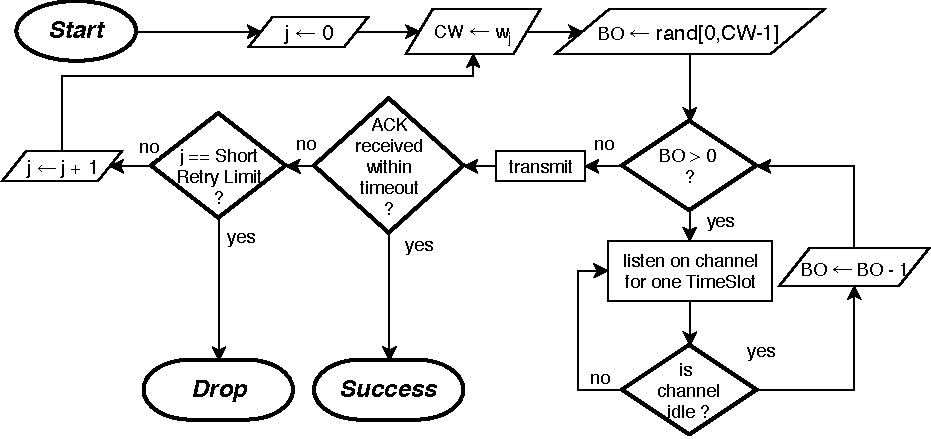
\includegraphics[width=0.8\textwidth]{images/ieee-80211-dcf.pdf}
\caption{Schematic flowgraph of the DCF, where $j$ is the current transmit attempt, $CW$ the current contention window size, $W_j$ the contention window size at attempt $j$ and $BO$ the back-off counter.}
\label{fig:dcfgraph}
\end{figure}


When nodes in a IEEE 802.11 network want to transmit data they must first
listen on the channel and wait until no activity has been detected for a
duration, the \emph{DCF Interframe Space} (DIFS). Since this effectively
synchronizes the nodes waiting to transmit, a random delay is introduced to
desynchronise nodes. This delay is called back-off time
($T_{\mathit{backoff}}$) and relates to the \emph{collision avoidance}
algorithm. The back-off procedure quantizes time into discrete
\emph{time-slots}, each $9$ $\mu$ to $50$ $\mu s$ long, depending on the IEEE
802.11 ``version''.

While in back-off, nodes listen on the medium for a full \emph{slot} and, if
no activity has been sensed, decrements the back-off counter. If nodes detect
activity on the medium during a slot, the counter is not decremented (counter
freezing). Upon reaching zero the node may attempt to (re)transmit. If no
\texttt{ACK} has been received after a certain duration (\texttt{ACK-Timeout})
the node waits another DIFS, enters further back-off and restarts its journey
back to zero again. The node has a fixed number of attempts to retransmit the
frame, \texttt{ShortRetryLimit} \cite{654749}, and drops the frame once
exceeded. The exponential increase of the back-off counter is visualised in
Figure \ref{fig:cwsizes}.

\begin{figure}
\center
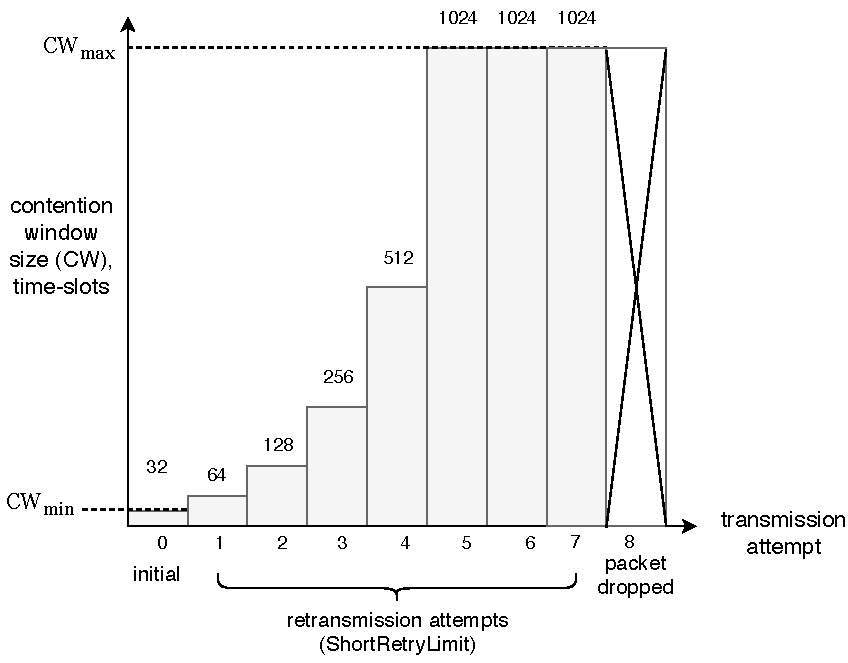
\includegraphics[width=0.8\textwidth]{images/contention-window-sizes.pdf}
\caption{Contention window size increases exponentially on each retransmission attempt, from $\mathit{CW}_{min}$ up to $\mathit{CW}_{max}$}
\label{fig:cwsizes}
\end{figure}

Time spent in back-off for each (re)transmission attempt $j$ is described in
equation \ref{eq:tbackoff}, where \emph{SlotTime} is defined in \cite{654749}
and $\mathcal{U}(0,W_j-1)$ is a uniformly sampled integer value between $0$
and the contention window size $W_{j}-1$, i.e., the maximum number of
time-slots (exclusive, since 0 is a valid back-off value).

\begin{equation} \label{eq:tbackoff}
T^j_{\mathit{backoff}} = \mathit{SlotTime} \times \mathcal{U}(0,W_j-1)
\end{equation}

The contention window configuration is commonly expressed by two parameters,
$CW_{min}$ and $CW_{max}$. As seen in Figure \ref{fig:cwsizes}, the initial
contention window size is $CW_{min}$ and each subsequent transmission attempt
will double the previous window size, with a maximum value $CW_{max}$. The
transmission attempt $m$ where the window size becomes $\mathit{CW}_{max}$ is
defined in Equation \ref{eq:mlog}.

\begin{equation} \label{eq:mlog}
m = \log_2 \frac{\mathit{CW}_{max}}{\mathit{CW}_{min}}
\end{equation}

Equation \ref{eq:cwj} defines the contention window size at attempt $j$, where
$L$ is the maximum number of retransmission attempts
(\texttt{ShortRetryLimit}). The defined values of $j$ are the initial attempt
($j=0$) and an extra $L$ attempts before termination, which resolves to $0
\leq j \leq L$.

\begin{equation} \label{eq:cwj}
W_j = \left\{
    \begin{array}{ll}
        2^j \mathit{CW}_{min}  & \mbox{if } 0 \leq j < m, \\
        \mathit{CW}_{max}      & \mbox{if } m \leq j \leq L
    \end{array}
\right.
\end{equation}

The description above details one of two relevant ``access modes'' (MACs) in
IEEE 802.11—``basic mode''. During CSMA/CA each node listens for activity
locally and can therefore fail to detect nodes whose signal is too weak to be
received, causing what's known as the \emph{hidden node} problem.

The second multiple access scheme requires that clients (also known as
stations or STAs) first acquire the right to transmit, using a \emph
{request-to-send} (RTS) message. If the STA is given permission, the AP will
respond with a \emph{clear-to-send} (CTS) message. This access scheme is
called RTS/CTS and potentially increases performance in scenarios with
multiple ``hidden nodes''. The RTS/CTS protocol assumes that all STAs  have
similar tx/rx capabilities. An overview of the required interframe spaces
(IFS) and protocol packets for ``basic'' and ``RTS/CTS'' modes and how they
compare, can be found in Figure \ref{fig:timings}.

\begin{figure}
\center
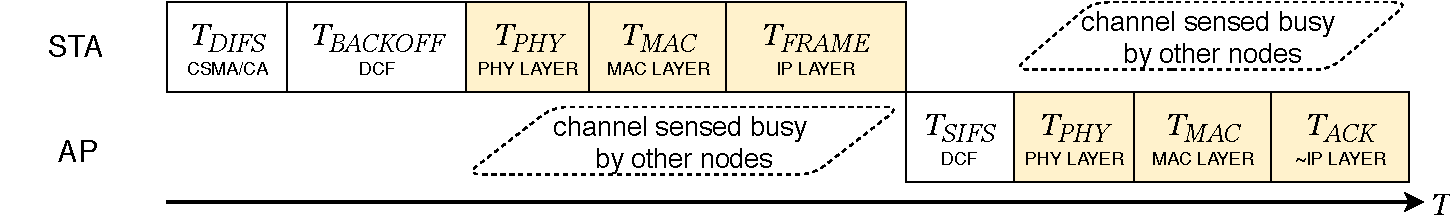
\includegraphics[width=0.8\textwidth]{images/time-overview.pdf}
\caption{Time overview of a successful frame transmission and response in ``basic mode'' and ``RTS/CTS mode''}
\label{fig:timings}
\end{figure}


\section{Linux Networking}

The Linux kernel has a complex networking subsystem which is beyond the scope
of this report to detail. Since we will be using Linux-based machines in our
tests and measurements, this section will present a refresh on the Linux
networking stack. Due to the measurements needed, only the outbound (egress)
path is described.

A high-level schematic view of a packet's path can be found in Figure \ref{fig:linux_egress}. It shows the packet's path from a userspace program,
through the kernel and into the network interface responsible for physically
transmitting it.  There are 5
main components in the figure: userspace, kernel, sockets, queueing
discipline (qdisc), driver and Network Interface Card (NIC). Each component is
more complex than described and interested readers are referred to
\cite{knet}, \cite{pcsending} and \cite[Chapter~17]{ldd}. The flow through
Figure \ref{fig:linux_egress} and the 5 components is described below:

\textbf{A userspace} program initializes, binds and attempts to send
data through a socket using system calls \texttt{socket(2)}, \texttt{bind(2)}
and \texttt{send(2)}, \texttt{sendto(2)} or \texttt{sendmsg(2)}.

\textbf{The linux kernel} allocates a per-socket kernel buffer
(\texttt{skb}),  where related kernel (bookkeeping), socket and packet data is
stored. The initial size of the \texttt{skb} depends on the
\texttt{net.core.wmem\_default} and  \texttt{net.core.wmem\_max} kernel
parameters. The \texttt{send(2)}, \texttt{sendto(2)} and  \texttt{sendmsg(2)}
syscalls must request memory from the \texttt{skb} belonging to the  socket
in use, before proceeding through the packet processing stack (UDP/TCP, IP,
etc)  and finally enqueuing the packet in the queueing discipline (qdisc). The
syscalls either blocks or fails, with \texttt{EWOULDBLOCK} or \texttt{EAGAIN},
when the  packet does not fit into the send buffer (\texttt{skb}), depending
on the I/O  mode of the socket (blocking or non-blocking).

\textbf{The queueing discipline} (qdisc) system is the internal
queueing system  of the linux kernel. A qdisc is a configurable, per-network
device queueing system with a  default ``pfifo\_fast'', prioritized fifo,
queue, see Figure \ref{fig:pfifofast}. As  packets arrive, the qdisc signals
the driver, using a scheduler, that data is available.  The qdisc can be
queried and configured using the \texttt{tc(8)} (traffic control),
\texttt{ip(8)} and \texttt{ifconfig(8)} programs. There is a reconfigurable
CPU core-to-qdisc mapping that specifies which CPUs can deliver packets to
a specific qdisc. This mapping can be configured using \texttt{ethtool(8)}.

\textbf{The driver} interfaces between the kernel and network device
hardware/firmware and can be considered a program itself (kernel module).
Drivers used throughout this thesis all use an internal ring buffer for egress
packets, called the ``TX-Ring''. The driver pulls packets from the qdisc into
the ``TX-Ring'' and signals the NIC that packets are ready to be sent. The
processing of freeing memory consumed by a packet is defered by an unknown
time after the NIC signals the driver it has processed the packet.

The Linux kernel supports a feature called ``packet taps'' which enable
kernel modules to capture packets as they enter or exit the kernel. The
outbound taps are called  at the end of the Linux kernel's outbound packet
processing path, right before control of  the packet is handed over to the
driver.

\textbf{The network interface card} (NIC) which primarily sends and
receives packets.  The internal design documents of many NICs are not publicly
available and open source drivers only hint at the design of important
subsystems, such as buffers and prefetchers.

The NICs used in this thesis are commonly found in laptops and do not
have a reconfigurable internal ``TX-Ring''. Common sense suggests that
NICs use some internal buffering mechanism in addition to the ``TX-Ring''
controlled by the driver. Since we have no way of differentiating between
these two ``TX-Rings'' the ``TX-Ring'' depicted in Figure
\ref{fig:linux_egress} should be seen as an abstraction of these two.


\begin{figure}
\center
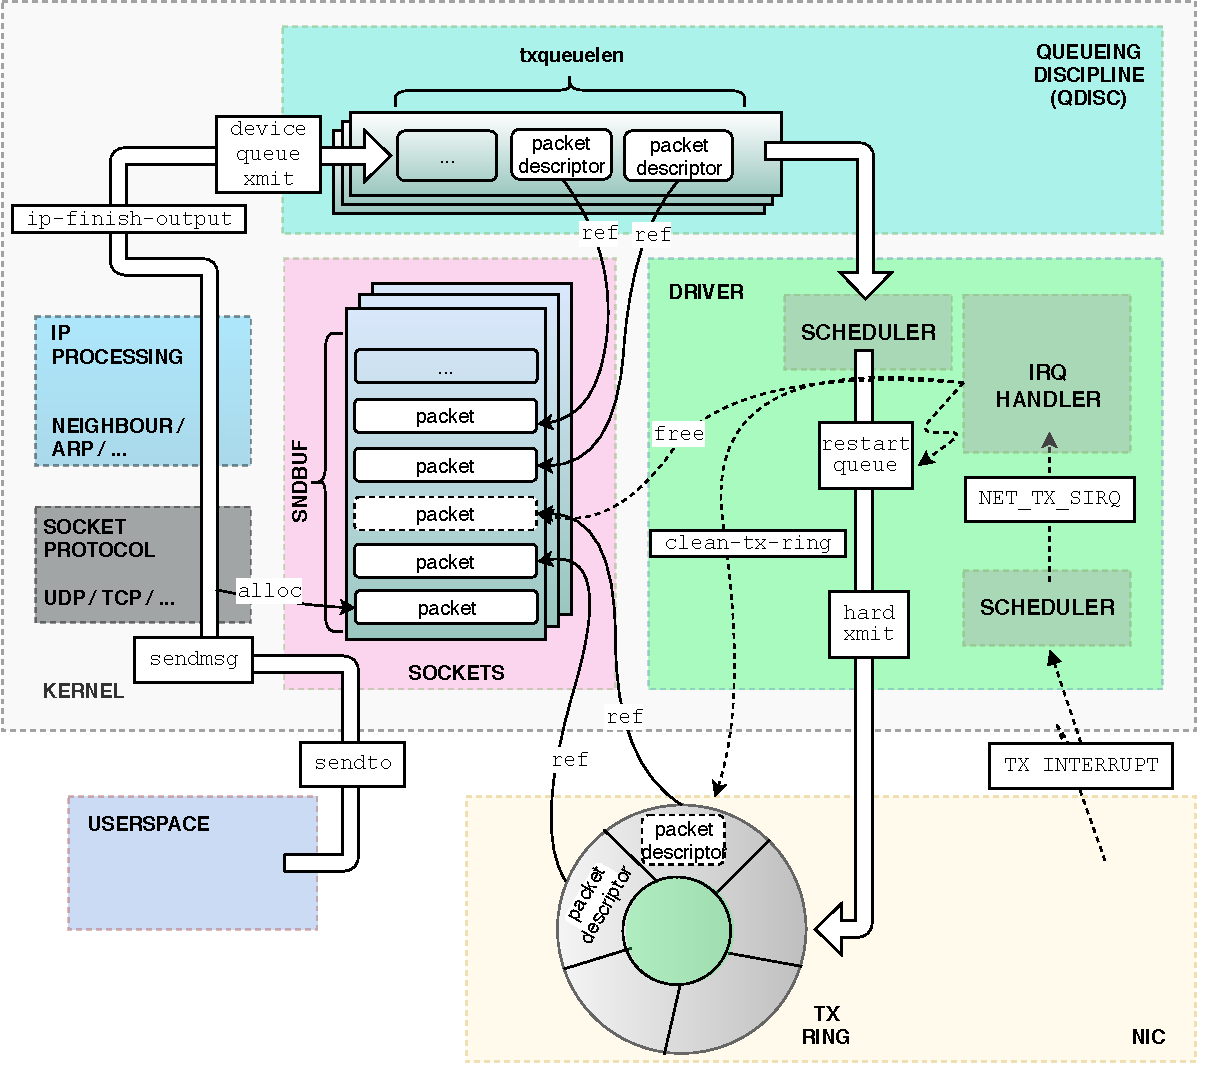
\includegraphics[width=0.9\textwidth]{images/linux-egress-overview.pdf}
\caption{Schematic overview of a packet's way from userspace to the physical network interface.}
\label{fig:linux_egress}
\end{figure}

\begin{figure}
\center
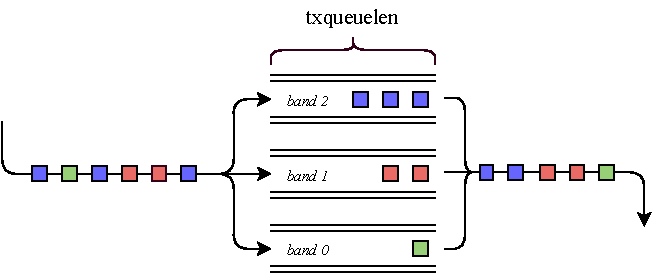
\includegraphics[width=0.8\textwidth]{images/pfifo-fast-queue.pdf}
\caption{An overview of the default queueing discipline, \texttt{pfifo\_fast}. Packets are enqueued into band 0, 1 or 2 depending on queue configuration and packet TOS bits. Band 0 is highest priority and band 2 lowest. Queue length is counted in number of packets.}
\label{fig:pfifofast}
\end{figure}

\section{Intel Wireless Wi-Fi Driver}

All selected machines used to measure Wi-Fi statistics have Intel wireless
network interface cards (NIC). On Linux these NICs are controlled by the ``Intel
Wireless WiFi driver for Linux''—\texttt{iwlwifi}.

The \texttt{iwlwifi} driver supports both an older operation mode, dvm
(\texttt{iwldvm}, as well as a newer, mvm (\texttt{iwlmvm}). The
\texttt{iwlmvm} module, included as part of \texttt{iwlwifi}, in the Linux
kernel source tree of version 4.13 was adapted for this thesis work to enable logging of packet timing statistics with microsecond accuracy.

Internally, the driver allocates a fixed number of ring buffers used for
holding transmission frame descriptors, firmware commands and incoming frames.
The memory of these ring buffers is shared between the host and the NIC by
using DMA controllers but resides in host DRAM. By using a ring buffer the
driver is able to queue up to 254 frame descriptors for transmission, and vice
versa for receiving. This design dramatically reduces the per-frame
communication overhead between driver and NIC in certain conditions, at the
expense of increased latency due to queueing.

\section{TG799-vac}

The OpenWrt-based router examined in this thesis, as depicted in Figure
\ref{fig:tg799} and commonly known as TG799-vac, supports two concurrent IEEE
802.11n and 802.11ac (2.4GHz and 5 GHz) IEEE 802.11 interfaces using 2x2 and
3x3 antenna configurations, respectively (tx-antennas x rx-antennas).  The
device is manufactured by Technicolor and uses Broadcom and Quantenna modems.

The IEEE 802.11n chip supports SGi (Short Guard interval) and STBC (Space-time
block code) over 20/40 MHz. The IEEE 802.11ac chip supports the same
technologies and increases the channel bandwidth to 20/40/80 MHz. SGi reduces
the guard interval used to eliminate intersymbol interference (as opposed to
interframe interference, which IFS eliminates) from 400 ns to 800 ns. STBC is
a technique to increase the reliability of transmission.

The router has been the default router provided by many Swedish ISPs and is
therefore a good router to use in the experiments. A custom firmware was used to gain root access, otherwise no particular changes were
made to keep the device in a ``natural'' condition, and should still be very
similar to any random installation.

\begin{figure}
\center
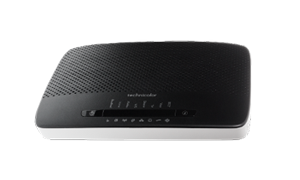
\includegraphics[width=0.5\textwidth]{images/tg799.png}
\caption{The TG799-vac router from Technicolor}
\label{fig:tg799}
\end{figure}

\section{ubus - the OpenWrt micro bus architecture}

\texttt{ubus} is command line interface to the bus daemon (\texttt{ubusd}).
Modules are organized by namespaces in \texttt{ubusd} and can be interacted 
with using \texttt{ubus}. A usage example can be found in Listing \ref{lst:ubusex}.

This tool was primarily used to read statistics from the TG799-vac device,
such as tx rates, packet counters and medium availability, intended for ``in
the wild'' evaluation of the model.

\begin{lstlisting}[language=bash,caption={ubus call listing all access points on this device},label=lst:ubusex]
$ ubus call wireless.accesspoint get
{
    "ap0": {
        "ssid": "wl0",
        "station_history": 1,
        "max_assoc": 0,
        ... (omitted)
    },
    "ap1": {
        ... (omitted)
    },
    ... (omitted)
}
\end{lstlisting}

A key observation is that output is encoded in JSON format, which does not limit
the size of numbers. Special care must be taken when using a JSON decoder to
ensure that numbers are deserialized correctly. We observed one such problem
during our thesis work.

\section{Wireshark}

Wireshark is a well-known program for capturing and inspecting network data,
and has been used extensively during the research and development of this
thesis. On Linux, it uses \texttt{libpcap} to register a packet tap for live
capture. Due to the way packet taps work in the Linux kernel Wireshark cannot
timestamp the moment the packet physically was transmitted, unless the network
interface card explicitly supports hardware timestamps. None of the NICs used
in this thesis have this feature, hence we cannot use Wireshark for any
time measurements.

\section{jana}

\texttt{jana} is a program, developed during this thesis, for running network
 tests. Specifically, network tests using expontential, uniform and gamma
 distributed packet send rates and payload sizes. This is in contrast to more
 powerful tools such as \texttt{pktgen} and \texttt{trafgen}, which offer
 better performance and more per-packet control at the expense of more
 configuration. Another widely used network benchmark tool is \texttt
 {iperf3}, which we used for some experiments. However, it does not--to our
 knowledge--support inter-packet latency and payload distributions.

As traffic patterns have a high impact on the network the idea was to see how
the model performed under bursty condition, such as web browsing and content
streaming, as well as constant-rate traffic such as video conferencing and
gaming.

The network test cycle is basically a ``ready, set, go!''-type of design: a
server waits for clients to say hello, and, after all $N$ clients have been
registered, broadcasts a ``set'' message which all clients echo back to the
server, which again waits for $N$ ``set'' before broadcasting a ``go''
message which marks the start of the network test. All clients wait
approximately 1 second after they have received the ``go'' message before
starting the packet generation, which decreases the likelihood of clients
failing to start due to the start packet being lost. This simple approach
proved resistant to partial network failures during the test wind-up stage.

The transmitting UDP socket was configured as non-blocking in an attempt to
emulate the inter-packet latency distribution as much as possible.

For interested readers, we recommend browsing the various
``Bufferbloat'' projects (\url{https://www.bufferbloat.net/projects/}), which
links to at least two very promising tools:

\texttt{IRTT} (\url{https://github.com/heistp/irtt}) -- ``IRTT measures round-trip time,
one-way delay and other metrics using UDP packets sent on a fixed period, and
produces both user and machine parseable output.''

\texttt{Flent} -- ``The FLExible Network Tester'' (\url{https://flent.org/}).
